

%%% outline
%-------------------------------------------------------------------------
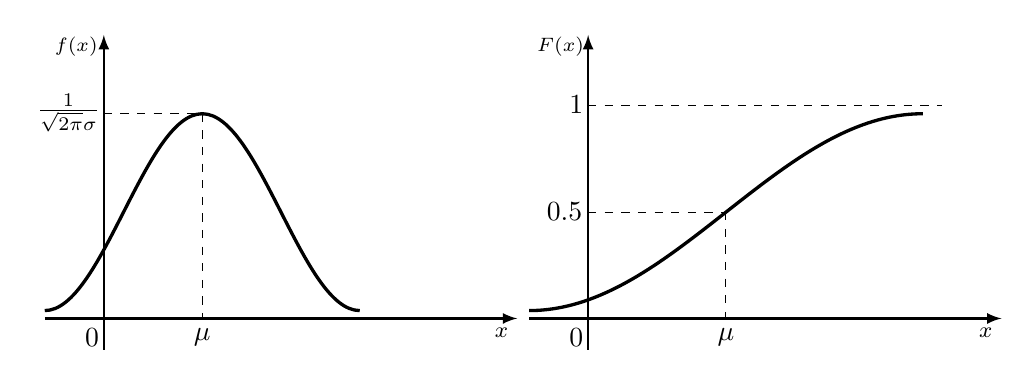
\begin{tikzpicture}


\begin{scope}[scale=0.5]

\draw [-,very thick] (-2,-1) cos(0,1.5) sin (2,4) cos(4,1.5) sin(6,-1) ;
\draw [-latex,thick] (-2.0,-1.2) -- (10,-1.2);%横轴
\draw [-latex,thick] (-0.5,-2.0) -- (-0.5,6);%纵轴
\draw [-,dashed] (2,4) -- (2,-1.2);  %%图中纵轴虚线
\draw [-,dashed] (-0.5,4) -- (2,4);  %%图中横轴虚线
\node [anchor=north] at (-0.8,-1.2) {0};
\node [anchor=north] at (2,-1.2) {$\mu$};
\node [anchor=north] at (-1.4,4.75) {$\frac{1}{\sqrt{2\pi}\sigma}$};
\node [anchor=north] at (-1.2,6.2) {\scriptsize{$f(x)$}};
\node [anchor=north] at (9.6,-1.2) {\footnotesize{$x$}};


\end{scope}

\begin{scope}[scale=0.5,xshift=35.0em]

\draw [-,very thick] (-2,-1) cos(3,1.5) sin(8,4) ;
\draw [-latex,thick] (-2.0,-1.2) -- (10,-1.2);%横轴
\draw [-latex,thick] (-0.5,-2.0) -- (-0.5,6.0);%纵轴
\draw [-,dashed] (3,1.5) -- (3,-1.2);  %%图中纵轴虚线
\draw [-,dashed] (-0.5,1.5) -- (3,1.5);  %%图中横轴虚线
\draw [-,dashed] (-0.5,4.2) -- (8.5,4.2);  %%图中横轴虚线
\node [anchor=north] at (-0.8,-1.2) {0};
\node [anchor=north] at (3,-1.2) {$\mu$};
\node [anchor=north] at (-1.1,2.0) {0.5};
\node [anchor=north] at (-0.8,4.7) {1};
\node [anchor=north] at (-1.2,6.2) {\scriptsize{$F(x)$}};
\node [anchor=north] at (9.6,-1.2) {\footnotesize{$x$}};

\end{scope}


\end{tikzpicture}
%---------------------------------------------------------------------



